\documentclass{standalone}
\usepackage{graphicx}	
\usepackage{amssymb, amsmath}
\usepackage{color}

\usepackage{tikz}
\usetikzlibrary{intersections, backgrounds, math}
\usepackage{pgfmath}

\definecolor{light}{RGB}{220, 188, 188}
\definecolor{mid}{RGB}{185, 124, 124}
\definecolor{dark}{RGB}{143, 39, 39}
\definecolor{highlight}{RGB}{180, 31, 180}
\definecolor{gray10}{gray}{0.1}
\definecolor{gray20}{gray}{0.2}
\definecolor{gray30}{gray}{0.3}
\definecolor{gray40}{gray}{0.4}
\definecolor{gray60}{gray}{0.6}
\definecolor{gray70}{gray}{0.7}
\definecolor{gray80}{gray}{0.8}
\definecolor{gray90}{gray}{0.9}
\definecolor{gray95}{gray}{0.95}

\begin{document}

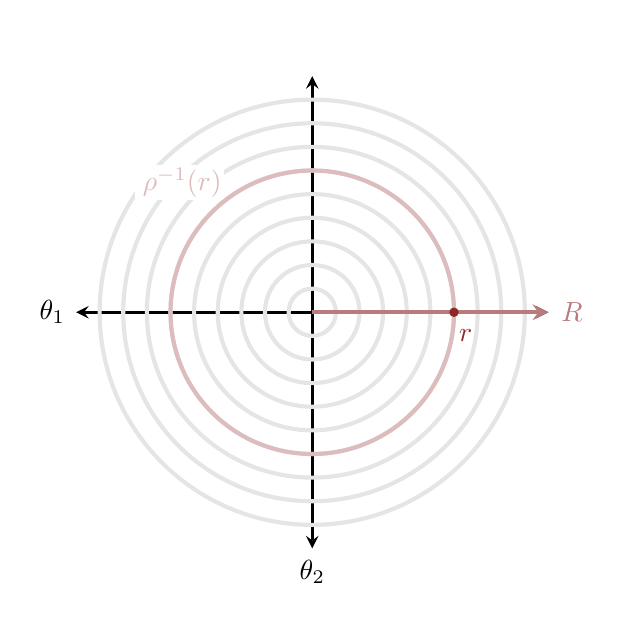
\begin{tikzpicture}[scale=0.3, thick]

\draw[white] (-12, -12) rectangle (12, 12);

\draw[<->, >=stealth, line width=1] (-10, 0) -- (10, 0);
\draw[<->, >=stealth, line width=1] (0, -10) -- (0, 10);

\node at (-11, 0) { $\theta_{1}$ };
\node at (0, -11) { $\theta_{2}$ };

\foreach \r in {1, 2, ..., 9} {
  \draw[gray90, line width=1.5] (0, 0) circle (\r);
}

\fill[white] (-7.5, 4.75) rectangle (-3.75, 6.25);
\node[light] at (-5.5, 5.5) { $\rho^{-1}(r)$ };

\draw[light, line width=1.5] (0, 0) circle (6);

\draw[->, >=stealth, line width=1.5, mid] (0, 0) -- (10, 0);
\node[mid] at (11, 0) { $R$ };

\fill[dark] (6, 0) circle (0.2);
\node[dark] at (6.5, -1) { $r$ };
  
\end{tikzpicture}

\end{document}  